% ---------------------------------------------------------------------------
%  Lecture slides -- Lab S2: Influence Lines (16:9, Beamer/metropolis)
%  Build: xelatex s2_slides.tex (twice)
% ---------------------------------------------------------------------------
\documentclass[aspectratio=169,11pt]{beamer}
\usetheme{metropolis}
\metroset{numbering=fraction,progressbar=frametitle,block=fill}
\usepackage{fontspec}\setsansfont{Latin Modern Sans}\usepackage{unicode-math}\setmathfont{Latin Modern Math}
\usepackage{amsmath,booktabs,array,siunitx,graphicx,tikz,multicol}
\graphicspath{{../figures/}}
% ---------------------------------------------------------------------------
%  s2figs.tex -- shared TikZ drawings for Lab S2 (Influence Lines)
%  Geometry in mm: A=0, B=250, C=440, D=690, E=880, F=1130.
%  \ILscale (cm per mm) is set by the including document before use.
% ---------------------------------------------------------------------------
\usetikzlibrary{arrows.meta,calc,patterns,decorations.pathreplacing}
\providecommand{\ILscale}{0.0115}
\colorlet{s2load}{orange!80!black}
\colorlet{s2reac}{blue!65!black}
\colorlet{s2hinge}{violet!80!black}
\colorlet{s2neg}{red!75!black}

% support symbols (anchored at beam centre line)
% offsets are given in cm so that the symbols keep their size whatever the x scale
\newcommand{\ILpin}[1]{%
  \draw[thick] (#1,-0.08) -- ++(-0.18cm,-0.3cm) -- ++(0.36cm,0) -- cycle;
  \draw[thick] ($(#1,-0.39)+(-0.26cm,0)$) -- ++(0.52cm,0);
  \foreach \t in {-0.22,-0.11,0,0.11,0.22} \draw ($(#1,-0.39)+(\t cm,0)$) -- ++(-0.08cm,-0.1cm);}
\newcommand{\ILroller}[1]{%
  \draw[thick] (#1,-0.08) -- ++(-0.18cm,-0.3cm) -- ++(0.36cm,0) -- cycle;
  \draw[thick] ($(#1,-0.45)+(-0.1cm,0)$) circle [radius=0.06cm] ($(#1,-0.45)+(0.1cm,0)$) circle [radius=0.06cm];
  \draw[thick] ($(#1,-0.52)+(-0.26cm,0)$) -- ++(0.52cm,0);
  \foreach \t in {-0.22,-0.11,0,0.11,0.22} \draw ($(#1,-0.52)+(\t cm,0)$) -- ++(-0.08cm,-0.1cm);}
\newcommand{\ILhingeat}[1]{\fill[white] (#1,0) circle [radius=0.11cm]; \draw[thick,s2hinge] (#1,0) circle [radius=0.11cm];}

% ---- the bridge model (elevation), with halts and span dimensions -----------
% optional argument: extra TikZ code drawn in the same picture (loads, arrows)
\newcommand{\ILbridge}[1][]{%
\begin{tikzpicture}[x=\ILscale cm,y=1cm,>=Stealth,font=\small]
  \pgfmathsetmacro{\xB}{250}\pgfmathsetmacro{\xC}{440}\pgfmathsetmacro{\xD}{690}\pgfmathsetmacro{\xE}{880}\pgfmathsetmacro{\xF}{1130}
  % beams
  \draw[line width=2.4pt] (0,0) -- (430,0);
  \draw[line width=2.4pt] (450,0) -- (680,0);
  \draw[line width=2.4pt] (700,0) -- (1130,0);
  \ILhingeat{440}\ILhingeat{690}
  \ILpin{0}\ILroller{250}\ILroller{880}\ILpin{1130}
  % halts
  \foreach \x/\l in {0/A,250/B,440/C,690/D,880/E,1130/F}
    \node[below,font=\small\bfseries] at (\x,-0.62) {\l};
  \foreach \x/\l in {100/1,200/2,300/3,400/4,500/5,600/6,700/7,800/8,900/9,1000/10,1100/11}
    {\draw (\x,-0.05) -- (\x,-0.22); \node[below,font=\scriptsize] at (\x,-0.22) {\l};}
  % dimensions
  \draw[|<->|] (0,-1.15) -- (250,-1.15) node[midway,below,font=\scriptsize] {250};
  \draw[|<->|] (250,-1.15) -- (440,-1.15) node[midway,below,font=\scriptsize] {190};
  \draw[|<->|] (440,-1.15) -- (690,-1.15) node[midway,below,font=\scriptsize] {250};
  \draw[|<->|] (690,-1.15) -- (880,-1.15) node[midway,below,font=\scriptsize] {190};
  \draw[|<->|] (880,-1.15) -- (1130,-1.15) node[midway,below,font=\scriptsize] {250};
  \node[font=\scriptsize,anchor=west] at (1140,-1.15) {mm};
  #1
\end{tikzpicture}}

% a downward load arrow at x (mm) with label
\newcommand{\ILload}[3][1.1]{\draw[->,very thick,s2load] (#2,#1) -- (#2,0.14) node[pos=0,above,font=\small\bfseries,s2load] {#3};}
% an upward reaction arrow at x with label (positive); negative drawn downward in red
\newcommand{\ILreaction}[3][0.9]{\draw[->,very thick,s2reac] (#2,-0.95-#1) -- (#2,-0.72) node[pos=0,below,font=\small,s2reac] {#3};}
\newcommand{\ILreactionneg}[3][0.9]{\draw[->,very thick,s2neg] (#2,-0.72) -- (#2,-0.95-#1) node[below,font=\small,s2neg] {#3};}

% ---- influence line plot: #1 = reaction name, #2 = list of x/y vertices -----
% #3 (optional) extra code; ordinate scale 1 unit = \ILyscale cm
\providecommand{\ILyscale}{1.0}
\newcommand{\ILilplot}[3][]{%
\begin{tikzpicture}[x=\ILscale cm,y=\ILyscale cm,>=Stealth,font=\small]
  \draw[gray!50,dashed] (250,-0.95) -- (250,1.95) (440,-0.95) -- (440,1.95) (690,-0.95) -- (690,1.95) (880,-0.95) -- (880,1.95);
  \draw[->] (0,0) -- (1180,0) node[right,font=\scriptsize] {$x$ (mm)};
  \foreach \x/\l in {0/A,250/B,440/C,690/D,880/E,1130/F} \node[below,font=\scriptsize\bfseries] at (\x,-0.02) {\l};
  \draw[very thick,s2reac] plot coordinates {#3};
  \node[anchor=south west,font=\small] at (0,1.5) {IL for #2};
  #1
\end{tikzpicture}}

% generated by s2_numbers.py / table script -- do not edit by hand
\newcommand{\TabOrdinates}{%
A & 0 & 1.000 & 0.000 & 0.000 & 0.000 & 0.000 & 0.000\\
1 & 100 & 0.600 & 0.400 & 0.000 & 0.000 & 0.000 & 0.000\\
2 & 200 & 0.200 & 0.800 & 0.000 & 0.000 & 0.000 & 0.000\\
B & 250 & 0.000 & 1.000 & 0.000 & 0.000 & 0.000 & 0.000\\
3 & 300 & -0.200 & 1.200 & 0.000 & 0.000 & 0.000 & 0.000\\
4 & 400 & -0.600 & 1.600 & 0.000 & 0.000 & 0.000 & 0.000\\
C & 440 & -0.760 & 1.760 & 1.000 & 0.000 & 0.000 & 0.000\\
5 & 500 & -0.578 & 1.338 & 0.760 & 0.240 & 0.422 & -0.182\\
6 & 600 & -0.274 & 0.634 & 0.360 & 0.640 & 1.126 & -0.486\\
D & 690 & 0.000 & 0.000 & 0.000 & 1.000 & 1.760 & -0.760\\
7 & 700 & 0.000 & 0.000 & 0.000 & 0.000 & 1.720 & -0.720\\
8 & 800 & 0.000 & 0.000 & 0.000 & 0.000 & 1.320 & -0.320\\
E & 880 & 0.000 & 0.000 & 0.000 & 0.000 & 1.000 & 0.000\\
9 & 900 & 0.000 & 0.000 & 0.000 & 0.000 & 0.920 & 0.080\\
10 & 1000 & 0.000 & 0.000 & 0.000 & 0.000 & 0.520 & 0.480\\
11 & 1100 & 0.000 & 0.000 & 0.000 & 0.000 & 0.120 & 0.880\\
F & 1130 & 0.000 & 0.000 & 0.000 & 0.000 & 0.000 & 1.000\\
}
\newcommand{\TabCompound}{%
A & 0 & 100 & 6.50 & 1.00\\
1 & 100 & 200 & 3.50 & 4.00\\
2 & 200 & 300 & 0.50 & 7.00\\
B & 250 & 350 & -1.00 & 8.50\\
3 & 300 & 400 & -2.50 & 10.00\\
4 & 400 & 500 & -4.44 & 11.34\\
C & 440 & 540 & -4.94 & 11.44\\
5 & 500 & 600 & -3.57 & 8.27\\
6 & 600 & 700 & -1.37 & 3.17\\
D & 690 & 790 & 0.00 & 0.00\\
}
\newcommand{\TabPracticeStudent}{%
A & 0 & 51 & & & \\
1 & 100 & 29 & & & \\
2 & 200 & 10 & & & \\
B & 250 & 1 & & & \\
3 & 300 & -11 & & & \\
4 & 400 & -28 & & & \\
C & 440 & -39 & & & \\
5 & 500 & -29 & & & \\
6 & 600 & -13 & & & \\
D & 690 & -1 & & & \\
7 & 700 & 0 & & & \\
8 & 800 & 0 & & & \\
E & 880 & 1 & & & \\
9 & 900 & -1 & & & \\
10 & 1000 & 0 & & & \\
11 & 1100 & 1 & & & \\
F & 1130 & 0 & & & \\
}
\newcommand{\TabPracticeKey}{%
A & 0 & 51 & 1.020 & 1.000 & +0.020 & +2.0\\
1 & 100 & 29 & 0.580 & 0.600 & -0.020 & -3.3\\
2 & 200 & 10 & 0.200 & 0.200 & 0.000 & +0.0\\
B & 250 & 1 & 0.020 & 0.000 & +0.020 & --\\
3 & 300 & -11 & -0.220 & -0.200 & -0.020 & -10.0\\
4 & 400 & -28 & -0.560 & -0.600 & +0.040 & +6.7\\
C & 440 & -39 & -0.780 & -0.760 & -0.020 & -2.6\\
5 & 500 & -29 & -0.580 & -0.578 & -0.002 & -0.3\\
6 & 600 & -13 & -0.260 & -0.274 & +0.014 & +5.1\\
D & 690 & -1 & -0.020 & 0.000 & -0.020 & --\\
7 & 700 & 0 & 0.000 & 0.000 & 0.000 & --\\
8 & 800 & 0 & 0.000 & 0.000 & 0.000 & --\\
E & 880 & 1 & 0.020 & 0.000 & +0.020 & --\\
9 & 900 & -1 & -0.020 & 0.000 & -0.020 & --\\
10 & 1000 & 0 & 0.000 & 0.000 & 0.000 & --\\
11 & 1100 & 1 & 0.020 & 0.000 & +0.020 & --\\
F & 1130 & 0 & 0.000 & 0.000 & 0.000 & --\\
}

\renewcommand{\ILscale}{0.0100}
\sisetup{per-mode=symbol}
\newcommand{\il}[1]{\eta_{#1}}
\definecolor{mAccent}{RGB}{31,111,178}
\setbeamercolor{progress bar}{fg=mAccent}
\setbeamercolor{title separator}{fg=mAccent}
\setbeamercolor{alerted text}{fg=orange!80!black}
\setbeamercolor{frametitle}{bg=black!80,fg=white}
\setbeamerfont{frametitle}{size=\large}
\setbeamertemplate{footline}{\hspace{3mm}{\tiny\color{black!50}\textcopyright\ 2026 Ahmad Razin Zainal Abidin and co-authors}\hfill{\scriptsize\color{black!50}SEAA 3012 CE Lab II -- Lab S2 Influence Lines\quad\insertframenumber/\inserttotalframenumber}\hspace{3mm}\vspace{2mm}}

\title{Influence Lines}
\subtitle{Lab S2 -- Cantilever (Gerber) Bridge Model}
\author{SEAA 3012 Civil Engineering Laboratory II}
\institute{Faculty of Civil Engineering, UTM}
\date{Revised edition, 2026\\[6pt]{\tiny\textcopyright\ 2026 Ahmad Razin Zainal Abidin and co-authors, Faculty of Civil Engineering, Universiti Teknologi Malaysia.\\ Free to share and adapt for non-commercial teaching and learning.}}

\begin{document}
\maketitle

% ----------------------------------------------------------------------------
\begin{frame}{Today}
\begin{columns}[T]
\column{0.55\textwidth}
\begin{enumerate}
  \item Why influence lines? What they are, what they are not
  \item The laboratory model and why it is determinate
  \item Deriving the six influence lines from statics
  \item The Müller--Breslau shortcut
  \item Using an influence line: one load, a train of loads, a distributed load
  \item The experiment: data reduction, errors, what to report
\end{enumerate}
\column{0.42\textwidth}
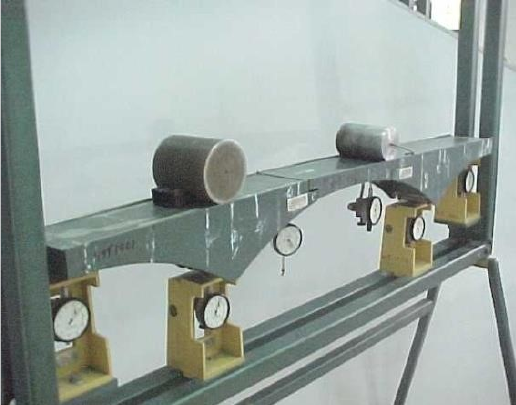
\includegraphics[width=\textwidth]{fig_s2_1}\\
{\scriptsize The bridge model in the Structures Laboratory.}
\end{columns}
\end{frame}

% ----------------------------------------------------------------------------
\section{Why influence lines?}
\begin{frame}{Loads that move}
\begin{columns}[T]
\column{0.6\textwidth}
A floor load stays put. A lorry on a bridge, a crane on its rail, a train on a viaduct do not.
\medskip

The designer needs to know \alert{where} the load must stand to produce
\begin{itemize}
  \item the largest reaction at a pier (bearing design, uplift),
  \item the largest shear at a section,
  \item the largest moment at midspan.
\end{itemize}
\medskip
A shear-force or bending-moment diagram cannot answer this: it assumes the loads are fixed.
\column{0.38\textwidth}
\begin{block}{Definition}
The \textbf{influence line} of a response $R$ at a fixed point is the graph of $R$ against the position $x$ of a \textbf{unit} load moving over the structure: ordinate $\il{R}(x)$, units of $R$ per unit load.
\end{block}
\end{columns}
\end{frame}

\begin{frame}{Influence line versus bending-moment diagram}
\begin{center}
\begin{tabular}{@{}p{3.3cm}p{4.6cm}p{4.6cm}@{}}
\toprule
 & SFD / BMD & Influence line\\
\midrule
Fixed & the loads & the point where $R$ is read\\
Varies along $x$ & the section where $V$, $M$ are read & the position of the unit load\\
Ordinate means & $V$ or $M$ at that section & $R$ at the fixed point for a load at $x$\\
\bottomrule
\end{tabular}
\end{center}
\medskip
Because the structure is linear elastic, effects add: once $\il{R}(x)$ is known for a unit load, \alert{any} load pattern is handled by multiplication and addition.
\end{frame}

% ----------------------------------------------------------------------------
\section{The laboratory model}
\begin{frame}{A Gerber (cantilever) bridge, 1130 mm long}
\begin{center}\ILbridge\end{center}
\begin{columns}[T]
\column{0.5\textwidth}
\begin{itemize}
  \item Beam ABC: pin A, roller B, cantilever BC (190 mm)
  \item Suspended span CD (250 mm) rests on \alert{hinges} at C and D
  \item Beam DEF: mirror image of ABC
\end{itemize}
\column{0.5\textwidth}
\begin{itemize}
  \item Gauges under A, B, E, F read the \alert{support reactions}
  \item Gauges under C, D read the \alert{hinge forces} (span pressing on the tips)
  \item Halts 1--11: where the mass is placed
\end{itemize}
\end{columns}
\end{frame}

\begin{frame}{Why it is statically determinate}
\begin{columns}[T]
\column{0.5\textwidth}
\textbf{Unknowns:} $R_A$, $R_B$, $R_E$, $R_F$ (no horizontal load, so no horizontal reactions) -- four.
\medskip

\textbf{Equations:}
\begin{itemize}
  \item $\sum F_y = 0$ and $\sum M = 0$ for the whole model -- two
  \item $M = 0$ at hinge C and at hinge D -- two more
\end{itemize}
Four equations, four unknowns.
\column{0.5\textwidth}
\begin{block}{Consequences}
\begin{itemize}
  \item Every reaction follows from equilibrium; $EI$ never appears.
  \item Every influence line is made of \alert{straight segments}, with kinks only at the hinges.
  \item Sign convention: reactions positive \emph{up}; $R_C$, $R_D$ positive when the span presses \emph{down} on the tip.
\end{itemize}
\end{block}
\end{columns}
\end{frame}

% ----------------------------------------------------------------------------
\section{Deriving the influence lines}
\begin{frame}{One idea, used three times: take moments about a support}
\begin{center}
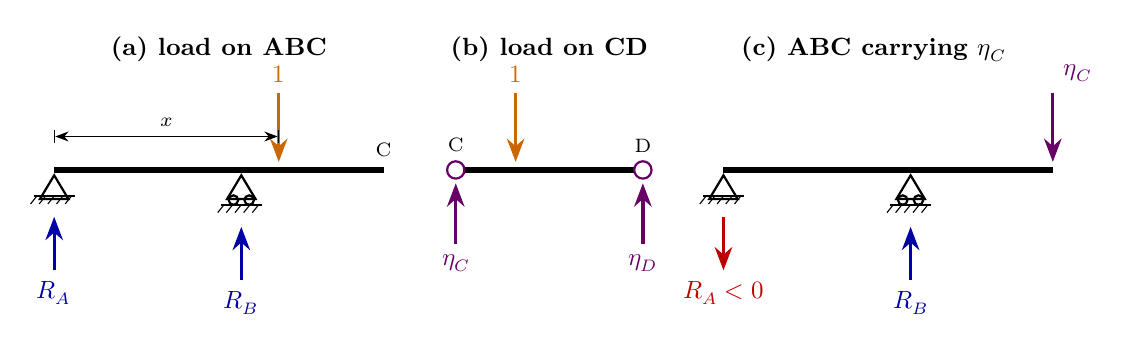
\begin{tikzpicture}[x=0.0095cm,y=0.85cm,>=Stealth,font=\small]
  \begin{scope}
    \draw[line width=2pt] (0,0) -- (440,0); \ILpin{0}\ILroller{250}
    \draw[->,very thick,s2load] (300,1.15) -- (300,0.12) node[pos=0,above,s2load] {$1$};
    \draw[->,very thick,s2reac] (0,-1.5) -- (0,-0.7) node[pos=0,below,s2reac] {$R_A$};
    \draw[->,very thick,s2reac] (250,-1.65) -- (250,-0.85) node[pos=0,below,s2reac] {$R_B$};
    \draw[|<->|] (0,0.5) -- (300,0.5) node[midway,above,font=\scriptsize] {$x$};
    \node[font=\small\bfseries] at (220,1.8) {(a) load on ABC};
    \node[above,font=\scriptsize] at (440,0.05) {C};
  \end{scope}
  \begin{scope}[xshift=5.1cm]
    \draw[line width=2pt] (0,0) -- (250,0); \ILhingeat{0}\ILhingeat{250}
    \node[above,font=\scriptsize] at (0,0.12) {C}; \node[above,font=\scriptsize] at (250,0.12) {D};
    \draw[->,very thick,s2load] (80,1.15) -- (80,0.12) node[pos=0,above,s2load] {$1$};
    \draw[->,very thick,s2hinge] (0,-1.1) -- (0,-0.2) node[pos=0,below,s2hinge] {$\il{C}$};
    \draw[->,very thick,s2hinge] (250,-1.1) -- (250,-0.2) node[pos=0,below,s2hinge] {$\il{D}$};
    \node[font=\small\bfseries] at (125,1.8) {(b) load on CD};
  \end{scope}
  \begin{scope}[xshift=8.5cm]
    \draw[line width=2pt] (0,0) -- (440,0); \ILpin{0}\ILroller{250}
    \draw[->,very thick,s2hinge] (440,1.15) -- (440,0.12) node[pos=0,above right,s2hinge] {$\il{C}$};
    \draw[->,very thick,s2neg] (0,-0.7) -- (0,-1.5) node[below,s2neg] {$R_A<0$};
    \draw[->,very thick,s2reac] (250,-1.65) -- (250,-0.85) node[pos=0,below,s2reac] {$R_B$};
    \node[font=\small\bfseries] at (200,1.8) {(c) ABC carrying $\il{C}$};
  \end{scope}
\end{tikzpicture}
\end{center}
\textbf{Order matters:} the suspended span is analysed first, because it is the only member whose loads reach the others.
\end{frame}

\begin{frame}{Step 1 -- load on beam ABC ($0 \le x \le 440$)}
Moments about B for beam ABC (hinge C unloaded):
\[
  R_A \cdot 250 - 1\cdot(250 - x) = 0 \quad\Longrightarrow\quad \il{A}(x) = \frac{250 - x}{250}, \qquad \il{B}(x) = 1 - \il{A} = \frac{x}{250}.
\]
\begin{columns}[T]
\column{0.55\textwidth}
\begin{itemize}
  \item Nothing stops at B: for $250 < x \le 440$ the lever arm $(250 - x)$ is \alert{negative}
  \item So $\il{A} < 0$: support A must \emph{hold the beam down}
  \item and $\il{B} > 1$: B carries the load \emph{and} the pull-down at A
\end{itemize}
\column{0.4\textwidth}
\begin{block}{At the tip C}
$\il{A}(440) = -190/250 = \mathbf{-0.76}$\\
$\il{B}(440) = 440/250 = \mathbf{1.76}$
\end{block}
\end{columns}
\end{frame}

\begin{frame}{Steps 2 and 3 -- load on the suspended span ($440 \le x \le 690$)}
\textbf{Step 2.} CD is a simply supported beam on the hinges (lever rule):
\[
  \il{C}(x) = \frac{690 - x}{250}, \qquad \il{D}(x) = \frac{x - 440}{250}, \qquad \il{C} + \il{D} = 1.
\]
\textbf{Step 3.} Beam ABC now carries only $\il{C}$ at its tip, i.e.\ Step 1 with the load standing at $x = 440$:
\[
  \il{A}(x) = -0.76\,\il{C}(x), \qquad \il{B}(x) = 1.76\,\il{C}(x).
\]
\begin{itemize}
  \item At C both formulae give $\il{A} = -0.76$: the line is \alert{continuous}
  \item At D, $\il{C} = 0$, hence $\il{A} = \il{B} = 0$: a load at D is carried entirely by DEF
\end{itemize}
\end{frame}

\begin{frame}{Step 4 -- load on beam DEF, and the checks}
\begin{columns}[T]
\column{0.5\textwidth}
DEF is the mirror image of ABC (E $\leftrightarrow$ B, F $\leftrightarrow$ A):
\[
  \il{F}(x) = \frac{x - 880}{250}, \quad \il{E}(x) = \frac{1130 - x}{250}
\]
for $690 \le x \le 1130$; for a load on CD, $\il{E} = 1.76\,\il{D}$ and $\il{F} = -0.76\,\il{D}$.
\medskip

A load on ABC never reaches DEF (and vice versa): the suspended span is unloaded and transmits nothing.
\column{0.48\textwidth}
\begin{block}{Three checks}
\begin{enumerate}
  \item $\il{A} + \il{B} + \il{E} + \il{F} = 1$ for every $x$
  \item Continuity at the hinges C and D
  \item Slopes: $-1/250$ per mm on ABC, $+0.76/250$ on CD; kinks only at hinges, \emph{never} at B
\end{enumerate}
\end{block}
\end{columns}
\end{frame}

\begin{frame}{The influence lines (1): the support reactions $R_A$ and $R_B$}
\begin{columns}[T]
\column{0.6\textwidth}
\renewcommand{\ILyscale}{0.72}\renewcommand{\ILscale}{0.0055}
\ILilplot[{\node[s2reac,font=\tiny,above left] at (0,1) {1.00};\node[s2neg,font=\tiny,below] at (440,-0.76) {$-0.76$};}]{$R_A$}{(0,1) (250,0) (440,-0.76) (690,0) (1130,0)}\\[4pt]
\ILilplot[{\node[s2reac,font=\tiny,above] at (440,1.76) {1.76};\node[s2reac,font=\tiny,above left] at (250,1) {1.00};}]{$R_B$}{(0,0) (250,1) (440,1.76) (690,0) (1130,0)}
\column{0.38\textwidth}
\small
\begin{tabular}{@{}c r r r@{}}
\toprule
Halt & $x$ & $\il{A}$ & $\il{B}$\\
\midrule
A & 0 & 1.00 & 0.00\\
1 & 100 & 0.60 & 0.40\\
2 & 200 & 0.20 & 0.80\\
B & 250 & 0.00 & 1.00\\
3 & 300 & $-0.20$ & 1.20\\
4 & 400 & $-0.60$ & 1.60\\
C & 440 & $-0.76$ & 1.76\\
5 & 500 & $-0.58$ & 1.34\\
6 & 600 & $-0.27$ & 0.63\\
D & 690 & 0.00 & 0.00\\
\bottomrule
\end{tabular}
\end{columns}
\end{frame}

\begin{frame}{The influence lines (2): hinge force $R_C$, and the right-hand side}
\begin{columns}[T]
\column{0.6\textwidth}
\renewcommand{\ILyscale}{0.72}\renewcommand{\ILscale}{0.0055}
\ILilplot[{\node[s2reac,font=\tiny,above] at (440,1) {1.00};}]{$R_C$ (hinge force)}{(0,0) (440,0) (440,1) (690,0) (1130,0)}\\[4pt]
\ILilplot[{\node[s2reac,font=\tiny,above] at (690,1.76) {1.76};\node[s2reac,font=\tiny,above right] at (880,1) {1.00};}]{$R_E$}{(0,0) (440,0) (690,1.76) (880,1) (1130,0)}
\column{0.38\textwidth}
\begin{itemize}
  \item $R_C$ is non-zero only for a load on the suspended span: a triangle, 1 at C, 0 at D
  \item $R_D$ is its mirror image (0 at C, 1 at D)
  \item $R_E$ and $R_F$ are the mirror images of $R_B$ and $R_A$ about $x = 565$ mm
  \item Reactions at B and E exceed the load (1.76) when it stands on the cantilever tips
\end{itemize}
\end{columns}
\end{frame}

% ----------------------------------------------------------------------------
\section{The Müller--Breslau principle}
\begin{frame}{The shortcut practising engineers use}
\begin{block}{Müller--Breslau (1886)}
Remove the restraint corresponding to $R$, impose a unit displacement in the direction of $R$: the \textbf{deflected shape} is the influence line of $R$.
\end{block}
\begin{center}
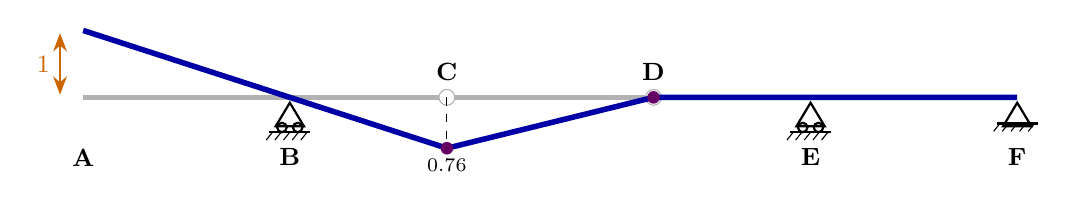
\begin{tikzpicture}[x=0.0105cm,y=0.85cm,>=Stealth,font=\small]
  \draw[gray!60,line width=1.6pt] (0,0) -- (430,0) (450,0) -- (680,0) (700,0) -- (1130,0);
  \draw[gray!60] (440,0) circle [radius=0.1cm] (690,0) circle [radius=0.1cm];
  \ILroller{250}\ILroller{880}\ILpin{1130}
  \draw[line width=2pt,s2reac] (0,1) -- (250,0) -- (440,-0.76) -- (690,0) -- (1130,0);
  \fill[s2hinge] (440,-0.76) circle [radius=0.08cm]; \fill[s2hinge] (690,0) circle [radius=0.08cm];
  \draw[<->,thick,s2load] (-28,0.04) -- (-28,0.96) node[midway,left,s2load] {1};
  \draw[dashed] (440,0) -- (440,-0.76) node[below,font=\scriptsize] {0.76};
  \foreach \x/\l in {0/A,250/B,880/E,1130/F} \node[below,font=\small\bfseries] at (\x,-0.62) {\l};
  \node[above,font=\small\bfseries] at (440,0.1) {C}; \node[above,font=\small\bfseries] at (690,0.1) {D};
\end{tikzpicture}
\end{center}
For $R_A$: release A, lift it by 1. ABC rotates about B as a rigid bar (C drops $190/250 = 0.76$); CD follows C and stays straight; DEF does not move. \alert{Same line, same signs}, no algebra.
\end{frame}

\begin{frame}{What the principle tells you at a glance}
\begin{columns}[T]
\column{0.5\textwidth}
\begin{itemize}
  \item Kinks only at hinges and at the released support -- a kink at B means an error
  \item Where the structure moves \emph{against} the released reaction, the ordinate is negative: uplift at A for a load between B and D
  \item Exact ordinates for \emph{determinate} structures (rigid links)
  \item Only the \emph{shape} for indeterminate ones: the released beam bends, the line is curved
\end{itemize}
\column{0.48\textwidth}
\begin{exampleblock}{Try it (Exercise 5)}
Sketch $\il{E}$ and $\il{F}$ by releasing E and F. Which supports can ever see uplift, and for which load positions?
\end{exampleblock}
\end{columns}
\end{frame}

% ----------------------------------------------------------------------------
\section{Using an influence line}
\begin{frame}{Three rules}
\begin{align*}
  R &= P\,\il{R}(x_1) && \text{single load $P$ at $x_1$}\\
  R &= \textstyle\sum_i P_i\,\il{R}(x_i) && \text{series of loads}\\
  R &= w \times (\text{area under the IL from $a$ to $b$}) && \text{uniform load $w$ on $[a,b]$}
\end{align*}
\begin{columns}[T]
\column{0.5\textwidth}
\begin{block}{Critical position}
All our ILs are piecewise linear, so $\sum_i P_i\,\il{R}(x_i)$ is piecewise linear in the position of the group: its extreme occurs with \alert{one load on a vertex} (A, B, C or D). Only a few positions need to be tried.
\end{block}
\column{0.48\textwidth}
\begin{block}{Units}
With masses in kg the reactions come out in kgf, which is what the gauges read ($1$ div $= 0.05$ kgf).
\end{block}
\end{columns}
\end{frame}

\begin{frame}{Worked example 1 -- the compound load of Test 2}
\SI{2.5}{kg} mass \SI{100}{mm} to the right of the \SI{5}{kg} mass (in front, moving right): $R_A(x) = 5\,\il{A}(x) + 2.5\,\il{A}(x + 100)$.
\begin{columns}[T]
\column{0.5\textwidth}
\begin{itemize}
  \item 5 kg mass at A: $5(1.0) + 2.5(0.6) = \mathbf{6.5}$ kgf
  \item 5 kg mass at C: $5(-0.76) + 2.5(-0.456) = \mathbf{-4.94}$ kgf
  \item 2.5 kg mass at C (5 kg at 340): $5(-0.36) + 2.5(-0.76) = -3.70$ kgf
\end{itemize}
The most severe pull-down occurs with the \alert{heavier} load on the vertex.
\column{0.46\textwidth}
\small
\begin{tabular}{@{}c r r r@{}}
\toprule
5 kg at & $x$ & $R_A$ (kgf) & $R_B$ (kgf)\\
\midrule
A & 0 & 6.50 & 1.00\\
1 & 100 & 3.50 & 4.00\\
2 & 200 & 0.50 & 7.00\\
B & 250 & $-1.00$ & 8.50\\
3 & 300 & $-2.50$ & 10.00\\
4 & 400 & $-4.44$ & 11.34\\
C & 440 & $-4.94$ & \textbf{11.44}\\
5 & 500 & $-3.57$ & 8.27\\
6 & 600 & $-1.37$ & 3.17\\
\bottomrule
\end{tabular}
\end{columns}
\end{frame}

\begin{frame}{Worked example 2 -- a uniformly distributed load}
Areas under $\il{A}$: $+125$ mm (AB), $-72.2$ mm (BC), $-95.0$ mm (CD), 0 (DEF).
\medskip

For $w = \SI{0.01}{kg/mm}$:
\begin{itemize}
  \item over AB only: $R_A = 0.01 \times 125 = 1.25$ kgf (half the load on a simple span)
  \item over BC and CD: $R_A = 0.01 \times (-167.2) = -1.67$ kgf
  \item over the \alert{whole model}: $R_A = 0.01 \times (-42.2) = -0.42$ kgf -- the deck \emph{lifts} at A
\end{itemize}
\medskip
\begin{block}{Check by statics}
ABC carries $w(250 + 190)$ directly plus $125w$ at C. Moments about B: $R_A \cdot 250 = 250w(125) - 190w(95) - 125w(190) = -10\,550w$, so $R_A = -42.2w$. The IL gave it without a new free-body diagram.
\end{block}
\end{frame}

% ----------------------------------------------------------------------------
\section{The experiment}
\begin{frame}{What you will do, and what the numbers mean}
\begin{columns}[T]
\column{0.5\textwidth}
\textbf{Test 1:} \SI{2.5}{kg} mass at each of the 17 halts; read all six gauges.\\
\textbf{Test 2:} \SI{5}{kg} + \SI{2.5}{kg} pair, \SI{100}{mm} apart.
\medskip

\begin{block}{Data reduction}
\[
  \il{\text{test}} = \frac{\text{reading (div)} \times 0.05}{m}, \qquad m = 2.5~\text{kg}
\]
Test 2: reading $\times\,0.05$ is the reaction in kgf.
\end{block}
\column{0.48\textwidth}
\textbf{Before leaving the lab}
\begin{itemize}
  \item Equilibrium check at every halt: $(a + b + e + f) \times 0.05 \approx 2.5$ kgf
  \item Re-zero the gauges between halts
  \item Centre the mass on the halt mark ($\pm 5$ mm matters)
\end{itemize}
\textbf{In the report:} theoretical and experimental ILs on the same axes, per reaction; absolute differences at every halt.
\end{columns}
\end{frame}

\begin{frame}{How good is ``good agreement''?}
\begin{columns}[T]
\column{0.58\textwidth}
\scriptsize
\begin{tabular}{@{}p{3.2cm}p{2.1cm}r@{}}
\toprule
Source & Estimate & on $\il{A}$\\
\midrule
Mass $\pm 5$ mm off the halt & slope $\times\,5$ mm & $\pm 0.020$\\
Gauge $\pm 1$ division & $0.05/2.5$ & $\pm 0.020$\\
Zero drift & re-zero each halt & $\pm 0.02$--$0.04$\\
Friction in hinges, gauges & systematic & sum check\\
\bottomrule
\end{tabular}
\medskip

Combined: about $\pm 0.03$ per unit load, the \alert{same at every halt}.
\column{0.4\textwidth}
\begin{alertblock}{Percentages mislead}
$\pm 0.03$ is 3\,\% of the ordinate at A (1.0) but 15\,\% at halt 2 (0.2), and undefined where the ordinate is zero.\\
Compare by \textbf{absolute difference}; quote percentages only at A, 1, 4, C, 5.
\end{alertblock}
\end{columns}
\end{frame}

% ----------------------------------------------------------------------------
\section{Activity and summary}
\begin{frame}{Activity: Influence Line Explorer}
\begin{columns}[T]
\column{0.64\textwidth}
Scan the code. \emph{Before each task}, write your prediction, then check it.
\begin{enumerate}
  \item Explorer, Part 1: the five tasks (read the reactions, open an explanation, set your own loads, find the critical position, use the areas).
  \item Explorer, Part 2: the five concept questions.
  \item After the laboratory: Exercises, worked by \textbf{hand calculation}; the Explorer only confirms.
  \item In the lab: type your gauge readings into the Lab tab and compare with theory before writing the report.
\end{enumerate}
\column{0.32\textwidth}
\centering

\includegraphics[width=0.78\linewidth]{qr_s2_explorer}\\[1pt]
{\scriptsize Influence Line Explorer}
\end{columns}
\end{frame}

\begin{frame}{Summary}
\begin{columns}[T]
\column{0.5\textwidth}
\begin{block}{Model: six straight-line influence lines}
$\il{A} = (250 - x)/250$ on ABC, $-0.76\,\il{C}$ on CD, 0 on DEF\\
$\il{B} = x/250$ on ABC, $1.76\,\il{C}$ on CD\\
$\il{C} = (690 - x)/250$, $\il{D} = (x - 440)/250$ on CD\\
$\il{E}$, $\il{F}$: mirror images of $\il{B}$, $\il{A}$\\
Check: $\il{A} + \il{B} + \il{E} + \il{F} = 1$
\end{block}
\column{0.48\textwidth}
\begin{block}{Use}
$R = \sum P_i\,\il{R}(x_i)$; UDL: $R = w \times$ area.\\
Extreme of a load train: one load on a vertex.\\
Müller--Breslau: release, displace by 1, read the shape.
\end{block}
\begin{block}{Report}
$\il{\text{test}} = \text{reading} \times 0.05/m$; equilibrium check; absolute differences; percentages only at large ordinates.
\end{block}
\end{columns}
\vspace{-6pt}
{\tiny Reading: Hibbeler, \emph{Structural Analysis}, 10th ed., ch.~6; Kassimali, \emph{Structural Analysis}, 6th ed., ch.~8; Laboratory Manual, experiment S2.}
\end{frame}
\end{document}
